\documentclass[12pt,a4paper]{report}

% Required packages
\usepackage[utf8]{inputenc}
\usepackage[T1]{fontenc}
\usepackage{geometry}
\usepackage{graphicx}
\usepackage{amsmath}
\usepackage{amsfonts}
\usepackage{amssymb}
\usepackage{hyperref}
\usepackage{cite}
\usepackage{fancyhdr}
\usepackage{titlesec}
\usepackage{tocloft}
\usepackage{listings}
\usepackage{xcolor}
\usepackage{booktabs}
\usepackage{array}
\usepackage{longtable}
\usepackage{float}
\usepackage{subcaption}
\usepackage{algorithm}
\usepackage{algpseudocode}
\usepackage{verbatim}
\usepackage{textcomp}
\usepackage{url}

\usepackage{enumitem}
\usepackage{booktabs}
\usepackage{pgfgantt}
\geometry{margin=1in}

% Page layout
\geometry{left=3cm, right=2.5cm, top=2.5cm, bottom=2.5cm}
\setlength{\parindent}{0pt}
\setlength{\parskip}{6pt}

% Code listing style
\lstset{
    basicstyle=\ttfamily\footnotesize,
    backgroundcolor=\color{gray!10},
    frame=single,
    numbers=left,
    numberstyle=\tiny,
    breaklines=true,
    captionpos=b,
    keywordstyle=\color{blue},
    commentstyle=\color{green!60!black},
    stringstyle=\color{red},
    showstringspaces=false,
    tabsize=2,
    escapeinside={(*@}{@*)}
}

% Header and footer
\pagestyle{fancy}
\fancyhf{}
\fancyhead[L]{\leftmark}
\fancyhead[R]{\thepage}
\renewcommand{\headrulewidth}{0.4pt}

% Hyperref configuration
\hypersetup{
    colorlinks=true,
    linkcolor=blue,
    filecolor=magenta,      
    urlcolor=cyan,
    citecolor=green,
    pdftitle={Facial Recognition System Documentation},
    pdfauthor={DEPI Development Team}
}

% Title page information
\title{\textbf{Facial Recognition System} \\ 
       \large Microsoft Machine Learning Project - Round 3 \\
       \large  CLS \\
       \large  ONL3\_AIS2\_S6 \\
       \large Project Documentation}
\author{Team members \\
        \vspace{0.5cm} \\
        \begin{tabular}{ll}
        21019073 & Basel Tarek Abdelmonsif \\
        21015768 & Mohammed Essam Shehata \\
        21016323 & Mostafa Sayed Salah \\
        21045220 & Naser Ali Naser \\
        21106079 & Zain Tamer Zain El-Abdin Awad \\
        \end{tabular}}
\date{}

\begin{document}

% Title page
\maketitle
\thispagestyle{empty}

\newpage

% Abstract
\chapter*{Abstract}
\addcontentsline{toc}{chapter}{Abstract}

This document contains the detailed documentation for the Microsoft Machine Learning Project Round 3 Facial Recognition project. The project uses cutting-edge deep learning architectures, such as FaceNet, VGGFace, and DeepFace models, to implement an end-to-end facial recognition system.

Five significant milestones are included in the system: (1) data collection and preprocessing through utilizing the LFW (Labeled Faces in the Wild) dataset. (2) model development with custom CNN architectures and pre-trained model fine-tuning; (3) deployment and testing via the streamlit app hosted by Hugging Face Server; (4) MLOps and monitoring implementation with MLflow and Kubeflow for continuous integration and model versioning; and (5) final documentation and performance analysis.

The system performs well, showing dependable face recognition in a range of environments, lighting conditions, and demographic groups. The model has demonstrated constant accuracy and stability through thorough testing, exhibiting resilient behavior even when put to the test with difficult real-world inputs. These outcomes demonstrate the efficacy of the suggested strategy and its applicability for real-world implementation.

The system is deployed using a web application based on Streamlit, which offers a user-friendly and interactive interface for real-time facial recognition. Hugging Face Spaces serves as the application's host, guaranteeing simple accessibility and smooth interaction with the machine learning pipeline underneath. As a fundamental resource for continued improvements and upcoming iterations of the facial recognition system, this documentation describes the architectural workflow, development methodology, and deployment strategy.

\textbf{Keywords:} Computer Vision, Deep Learning, FaceNet, Facial Recognition, MLOps, OpenCV, VGGFace

\newpage

% Table of Contents
\tableofcontents

\newpage

% Chapter 1
\chapter{Project Planning & Management}

\section{Project Overview}

The Facial Recognition System project is a thorough application of modern machine learning and computer vision technologies to produce a reliable, scalable, and production-ready facial recognition system. The integration of state-of-the-art deep learning models with enterprise-grade deployment infrastructure was the main focus of this project, which was created as part of the Microsoft Machine Learning Project Round 3.

In a number of fields, such as identity verification, access control, security systems, and customized user experiences, facial recognition technology has grown in significance. This project tackles the difficulties of creating a system that, in addition to achieving high accuracy, preserves scalability, dependability, and ethical considerations in practical applications.

\section{Objectives}

The primary objectives of this facial recognition system project are:

\begin{itemize}
    \item \textbf{High Accuracy Implementation:} Develop a facial recognition system achieving high accuracy rates
    \item \textbf{Modern ML Pipeline:} Implement comprehensive MLOps practices including automated testing, model versioning, and continuous integration
    \item \textbf{Production usage:} Build ready web app for deployment with proper model usage and monitoring capabilities
    \item \textbf{Performance Optimization:} Optimize response speed and resource utilization as much as possible to run the project in real time
\end{itemize}

\section{Scope and Limitations}

\subsection{Project Scope}

The project encompasses the following components:

\begin{enumerate}
    \item \textbf{Data Pipeline:} Complete data collection, preprocessing, and augmentation pipeline using the LFW dataset
    \item \textbf{Model Development:} Implementation and comparison of multiple deep learning architectures including FaceNet, VGGFace, and custom CNN models
    \item \textbf{Model deployment:} Run a Streamlit web app that uses the trained model for monitoring and predictions.
    \item \textbf{MLOps Infrastructure:} Comprehensive monitoring and deployment pipeline using MLflow and Kubeflow
    \item \textbf{Performance Analysis:} Detailed evaluation using standard metrics for different groups
\end{enumerate}

\subsection{Limitations}

\begin{itemize}
    \item The system is trained primarily on the LFW dataset, which may limit generalization to certain demographic groups
    \item Real-time processing is optimized for single-face scenarios; multi-face detection requires additional processing time
    \item The current implementation focuses on face verification rather than identification from large databases
\end{itemize}

% #////////////////////////////////////////////////////////////////

\newpage
\section{Project Plan}

\subsection{Timeline (Gantt Chart)}
\begin{figure}[htbp]
\centering
\resizebox{\textwidth}{!}{%
\begin{ganttchart}[
    hgrid,
    vgrid,
    x unit=0.6cm, % Reduced x unit
    y unit chart=0.8cm,
    bar/.append style={fill=blue!50},
    milestone/.append style={fill=red!50}
]{1}{12}
\gantttitle{Project Timeline}{12} \\
\gantttitlelist{1,...,12}{1} \\

% Phase 1
\ganttgroup{Phase 1: Data Pipeline}{1}{4} \\
\ganttbar[name=setup]{Project Setup}{1}{1} \\
\ganttbar[name=data]{Data Collection \& Preprocessing}{1}{3} \\
\ganttbar[name=aug]{Data Augmentation}{3}{4} \\
\ganttmilestone[name=p1done]{P1 Complete}{4} \\

% Phase 2
\ganttgroup{Phase 2: Model Development}{4}{8} \\
\ganttbar[name=models]{Implement Models}{4}{7} \\
\ganttbar[name=eval]{Model Evaluation}{7}{8} \\
\ganttmilestone[name=p2done]{P2 Complete}{8} \\

% Phase 3
\ganttgroup{Phase 3: Deployment \& MLOps}{8}{11} \\
\ganttbar[name=app]{Streamlit App}{8}{10} \\
\ganttbar[name=mlops]{MLOps}{9}{11} \\
\ganttmilestone[name=p3done]{P3 Complete}{11} \\

% Phase 4
\ganttgroup{Phase 4: Analysis \& Docs}{11}{12} \\
\ganttbar[name=analysis]{Performance Analysis}{11}{12} \\
\ganttbar[name=docs]{Final Documentation}{11}{12} \\
\ganttmilestone[name=p4done]{Project Complete}{12} \\

% Links
\ganttlink{data}{aug}
\ganttlink{models}{eval}
\ganttlink{app}{mlops}
\ganttlink{p3done}{analysis}
\end{ganttchart}%
}
\caption{Project Timeline and Milestones}
\end{figure}

\subsection{Milestones and Deliverables}
\begin{itemize}
    \item \textbf{Data Pipeline Complete (End of Week 4):} The result of this phase is a fully functional data processing pipeline and the data are ready to be used.
    \item \textbf{Model Development (End of Week 8):} Deliverable includes trained models and a comparative analysis report.
    \item \textbf{Deployment Complete (End of Week 11):} Results are the deployed Streamlit web app and the configured MLOps infrastructure.
    \item \textbf{Project Complete (End of Week 12):} Final deliverables include a performance analysis report, full project documentation, and presentation materials.
\end{itemize}

\subsection{Resource Allocation}
\begin{table}[htbp]
\centering
\begin{tabular}{lp{0.6\textwidth}}
\toprule
\textbf{Resource} & \textbf{Approximate Usage / Notes} \\
\midrule
Cloud GPU Instances & Moderate usage for training multiple deep learning models over an 8-week period. \\
\hline
Cloud Storage & Moderate usage for the LFW dataset, augmented data, and model artifacts. \\
\hline
Hugging Face Spaces & Hosting for the Streamlit-based web application for demonstration and predictions. \\
\hline
MLOps Infrastructure & MLflow for experiment tracking and Kubeflow for pipeline automation. Self-hosted or managed services. \\
\hline
Development Environments & Local machines for 5 team members for coding and testing. \\
\bottomrule
\end{tabular}
\caption{Resource Allocation Summary}
\end{table}


\section{Task Assignment \& Roles}
\begin{table}[htbp]
\centering
\resizebox{\textwidth}{!}{%
\begin{tabular}{l|p{0.25\textwidth}|p{0.25\textwidth}|p{0.25\textwidth}|p{0.25\textwidth}}
\toprule
\textbf{Member} & \textbf{Phase 1: Data Pipeline} & \textbf{Phase 2: Model Development} & \textbf{Phase 3: Deployment \& MLOps} & \textbf{Phase 4: Analysis \& Docs} \\
\midrule
\textbf{Member 1} & Project planning \& coordination. Lead data collection efforts. & Implement FaceNet model. & Optimize the final model for deployment. & Lead performance analysis and compile the final project report. \\
\hline
\textbf{Member 2} & Participated in data preprocessing. & Supervise model development and set up evaluation methods. & Assist with integrating the selected model into the Streamlit app. & Analyze and report on some performance metrics. \\
\hline
\textbf{Member 3} & Participated in data preprocessing. & Implement VGGFace model. & Coordinate deployment activities and system integration. & Analyze and report on some performance metrics. \\
\hline
\textbf{Member 4} & Participated in data augmentation & Compared between different models metrics & Build and manage the MLOps pipeline for automated training and deployment. & Lead performance analysis and compile the final project report. \\
\hline
\textbf{Member 5} & Participated in data augmentation & Contributed the results to the custom model. & Develop and test the Streamlit web application on Hugging Face Spaces. & Conduct system-wide testing and prepare user documentation. \\
\bottomrule
\end{tabular}%
}
\caption{Team Roles and Responsibilities by Project Phase}
\end{table}


\section{Risk Assessment \& Mitigation Plan}
\begin{table}[htbp]
\centering
\begin{tabular}{lp{0.6\textwidth}}
\toprule
\textbf{Risk} & \textbf{Mitigation Strategy} \\
\midrule
Bad model performance & Use pre-trained models as a starting point then perform hyperparameter tuning and apply data augmentation to enhance the results. \\
\hline
Schedule delays & When feasible, complete tasks in parallel, set aside time for important tasks, and conduct weekly progress meetings. \\
\hline
Team member unavailability & Provide members with additional instruction on important duties and keep thorough, collaborative documentation. \\
\bottomrule
\end{tabular}
\caption{Key Risks and Mitigation Strategies}
\end{table}

\section{Key Performance Indicators (KPIs)}
\begin{table}[htbp]
\centering
\begin{tabular}{llc}
\toprule
\textbf{Category} & \textbf{KPI} & \textbf{Target} \\
\midrule
System Performance & System Uptime & $\geq 99\%$ \\

\midrule
Model Performance & Recognition Accuracy & $\geq 90\%$ \\
& Inference Time & $\leq 500$ ms \\
\bottomrule
\end{tabular}
\caption{Key Performance Indicators}
\end{table}
% #////////////////////////////////////////////////////////////////

\newpage
\chapter{Literature Review}
\label{chap:literature_review}

\section{Overview of Facial Recognition Systems}

From conventional computer vision methods to deep learning strategies employing CNNs, facial recognition has changed over time. On benchmark datasets, contemporary systems attain nearly human accuracy while managing real-world obstacles like changing lighting, pose, and environmental challenges.


\subsection{LFW Dataset}

The Labeled Faces in the Wild (LFW) dataset  is the standard benchmark for face verification, containing 13,233 images of 5,749 individuals. It presents realistic challenges with variations in pose, lighting, expression, and resolution.

\section{Deep Learning Architectures}

\subsection{FaceNet}

FaceNet uses triplet loss to map faces to 128-dimensional embeddings where Euclidean distance represents face similarity. It achieves 99.63\% accuracy on LFW using Inception-based architectures.

\subsection{VGGFace}

VGGFace uses VGG-16 architecture for face recognition, generating 4,096-dimensional descriptors. VGGFace2 improves performance using ResNet architectures.

\subsection{Custom CNN Architectures}

Recent innovations include ArcFace (angular margin loss), MobileFaceNet (lightweight for mobile), and CosFace (cosine margin loss), each optimizing for specific deployment scenarios.

\begin{table}[h]
\centering
\caption{Architecture Comparison}
\label{tab:architecture_comparison}
\begin{tabular}{|l|c|c|c|}
\hline
\textbf{Architecture}  & \textbf{Parameters} & \textbf{Embedding Size} \\
\hline
FaceNet  & 23M & 128 \\
VGGFace2 (ResNet-50)  & 25M & 2048 \\
ArcFace (ResNet-100) & 65M & 512 \\
MobileFaceNet & 1M & 128 \\
\hline
\end{tabular}
\end{table}

\section{Data Preprocessing \& Augmentation}

Face alignment and detection To find facial landmarks and adjust posture, utilize MTCNN or Dlib. To increase robustness, data augmentation techniques include color corrections, noise injection, and geometric transformations (rotation, scaling, and flipping). Generalization is improved by sophisticated methods like MixUp and CutMix.

\section{MLOps Infrastructure}

\subsection{MLflow}
MLflow offers deployment management, model versioning, and experiment tracking. It records metrics, artifacts, and parameters for systematic model comparison and repeatable experiments.

\subsection{Kubeflow}
Model serving, pipeline definition, distributed training, and production monitoring are all supported by Kubeflow, which orchestrates machine learning workflows on Kubernetes.

\subsection{Streamlit \& Hugging Face}
Streamlit makes it possible to quickly create interactive machine learning applications using Python. Hugging Face Spaces offers easy deployment, GPU support, and Git integration for free hosting.

\section{Evaluation Metrics}

\textbf{Classification Metrics:} Accuracy, Precision, Recall, F1-Score, FAR (False Acceptance Rate), FRR (False Rejection Rate)

\textbf{ROC-AUC:} Area under ROC curve; AUC > 0.9 indicates excellent performance

\textbf{EER:} Equal Error Rate where FAR = FRR; lower is better (SOTA < 0.1\%)


\textbf{Deployment Metrics:} Response time, throughput, system uptime, resource utilization

\section{Suggested Improvements}
\subsection{Technical Enhancements}

\begin{enumerate}
    \item \textbf{Model Architecture}: Include ensemble techniques, multi-task learning, and attention mechanisms.
    \item \textbf{Training}: Use adaptive learning rates, advanced loss functions (ArcFace, CosFace).
\end{enumerate}

\subsection{Fairness \& Ethics}

\begin{enumerate}
    \item \textbf{Bias Mitigation}: Balance dataset demographics, fairness-aware training, continuous auditing
    \item \textbf{Privacy}: Data anonymization, consent management, liveness detection for anti-spoofing
\end{enumerate}

%///////////////////////////////////////////////////////

\chapter{Requirements Gathering}

\section{Stakeholder Analysis}

\begin{table}[h]
\centering
\caption{Key Stakeholders and Their Needs}
\label{tab:stakeholders}
\begin{tabular}{|l|p{5cm}|p{5cm}|}
\hline
\textbf{Stakeholder} & \textbf{Role} & \textbf{Primary Needs} \\
\hline
End Users & Security personnel, operators & Accurate recognition, easy interface \\
Data Scientists & Model developers & Experiment tracking, model comparison \\
Administrators & IT personnel & System monitoring, maintenance \\
Management & Decision makers & Reliability, compliance, reporting \\
\hline
\end{tabular}
\end{table}

\section{User Stories \& Use Cases}

\subsection{User Stories}

\begin{itemize}
    \item \textbf{US1}: As an end user, I want to upload face images and get verification results quickly
    \item \textbf{US2}: As a data scientist, I want to compare multiple models to select the best one
    \item \textbf{US3}: As an administrator, I want to monitor system performance in real-time
\end{itemize}

\subsection{Key Use Case: Face Verification}

\begin{itemize}
    \item \textbf{Actor}: End User
    \item \textbf{Flow}: Upload image → Detect face → Generate embedding → Compare with database → Return result
    \item \textbf{Output}: Verification result with confidence score
\end{itemize}

\section{Functional Requirements}

\begin{table}[h]
\centering
\caption{Functional Requirements}
\label{tab:functional_requirements}
\begin{tabular}{|l|p{9cm}|}
\hline
\textbf{ID} & \textbf{Requirement} \\
\hline
FR1 & Face detection and alignment from input images \\
FR2 & Face verification using FaceNet, VGGFace, and Custom CNN \\
FR3 & Model training with experiment tracking (MLflow) \\
FR4 & Web interface using Streamlit \\
FR5 & Performance metrics visualization and fairness evaluation \\
FR6 & Batch processing and result export \\
\hline
\end{tabular}
\end{table}

\section{Non-functional Requirements}

\subsection{Performance}
\begin{itemize}
    \item Response time < 5 seconds per image
    \item Model accuracy > 90\% on LFW dataset
\end{itemize}

\subsection{Security \& Privacy}
\begin{itemize}
    \item Data is hidden for model training
\end{itemize}

\subsection{Usability \& Reliability}
\begin{itemize}
    \item Simple interface
    \item High system uptime
    \item Browser compatibility (Chrome, Firefox, Safari, Edge)
\end{itemize}

\subsection{Deployment}
\begin{itemize}
    \item Hosted on Hugging Face Spaces
    \item Automated CI/CD pipeline
\end{itemize}

\chapter{System Analysis \& Design}
\label{chap:system_design}

\section{Problem Statement \& Objectives}

\subsection{Problem Statement}

There are different challenges facing traditional facial recognition systems:
\begin{itemize}
    \item Limited detail on unrestricted real-world photos with different lighting and postures
    \item Absence of thorough frameworks for comparing various architectures
    \item Potential bias across demographic groups affecting fairness
\end{itemize}

\subsection{Project Objectives}

\begin{enumerate}
    \item \textbf{Develop Robust Recognition System}: Implement and compare FaceNet, VGGFace, and custom CNN architectures achieving >90\% accuracy on LFW dataset
    
    \item \textbf{Build Complete Data Pipeline}: Create preprocessing and augmentation pipeline for LFW dataset with face detection and alignment
    
    \item \textbf{Establish MLOps Infrastructure}: Implement experiment tracking with MLflow and orchestration with Kubeflow
    
    \item \textbf{Deploy Simple Interactive Web App}: Develop Streamlit web application hosted on Hugging Face Spaces
    
    \item \textbf{Ensure Fairness}: Evaluate and mitigate bias across demographic groups as much as possible
\end{enumerate}

\section{Use Case Diagram \& Descriptions}

\subsection{System Actors}

\begin{itemize}
    \item \textbf{End User}: Uploads images for face verification
    \item \textbf{Data Scientist}: Trains and evaluates models
    \item \textbf{System Administrator}: Monitors and maintains system
    \item \textbf{External System}: Integrates via API (optional)
\end{itemize}

\subsection{Primary Use Cases}

\begin{figure}[h]
\centering
\begin{tikzpicture}[node distance=2cm]
% Actors
\node (user) [actor] {End User};
\node (ds) [actor, below=of user] {Data Scientist};
\node (admin) [actor, below=of ds] {Admin};

% Use Cases (positioned to the right)
\node (verify) [usecase, right=3cm of user] {Verify Face};
\node (batch) [usecase, below=0.5cm of verify] {Batch Process};
\node (train) [usecase, right=3cm of ds] {Train Model};
\node (compare) [usecase, below=0.5cm of train] {Compare Models};
\node (monitor) [usecase, right=3cm of admin] {Monitor System};
\node (deploy) [usecase, below=0.5cm of monitor] {Deploy Model};

% Connections
\draw (user) -- (verify);
\draw (user) -- (batch);
\draw (ds) -- (train);
\draw (ds) -- (compare);
\draw (admin) -- (monitor);
\draw (admin) -- (deploy);
\end{tikzpicture}
\caption{Use Case Diagram}
\label{fig:use_case}
\end{figure}


\subsection{Use Case Descriptions}

\subsubsection{UC1: Verify Face}
\begin{itemize}
    \item \textbf{Actor}: End User
    \item \textbf{Description}: User uploads image for face verification against database
    \item \textbf{Precondition}: User has access to web interface
    \item \textbf{Flow}: Upload → Detect → Align → Extract features → Match → Display result
    \item \textbf{Postcondition}: Verification result with confidence score displayed
\end{itemize}

\subsubsection{UC2: Train Model}
\begin{itemize}
    \item \textbf{Actor}: Data Scientist
    \item \textbf{Description}: Train new model architecture with specified hyperparameters
    \item \textbf{Precondition}: Dataset preprocessed and ready
    \item \textbf{Flow}: Configure → Train → Log metrics → Evaluate → Register model
    \item \textbf{Postcondition}: Model saved in registry with performance metrics
\end{itemize}

\subsubsection{UC3: Monitor System}
\begin{itemize}
    \item \textbf{Actor}: Administrator
    \item \textbf{Description}: Monitor system health and performance metrics
    \item \textbf{Precondition}: System deployed and operational
    \item \textbf{Flow}: Access dashboard → View metrics → Check alerts → Take action
    \item \textbf{Postcondition}: System status understood, actions logged
\end{itemize}

\section{Functional \& Non-Functional Requirements}

\subsection{Functional Requirements}

\begin{table}[h]
\centering
\caption{Functional Requirements Summary}
\label{tab:func_req_summary}
\begin{tabular}{|l|p{10cm}|}
\hline
\textbf{ID} & \textbf{Requirement} \\
\hline
FR1 & Detect and align faces from input images using MTCNN \\
FR2 & Extract face embeddings using FaceNet, VGGFace, Custom CNN \\
FR3 & Compare embeddings and return similarity scores \\
FR4 & Train models with configurable hyperparameters \\
FR5 & Track experiments using MLflow (params, metrics, artifacts) \\
FR6 & Deploy models via Streamlit web interface \\
FR7 & Process single images and batches \\
FR8 & Visualize performance metrics (accuracy, ROC, confusion matrix) \\
\hline
\end{tabular}
\end{table}

\subsection{Non-Functional Requirements}

\begin{table}[h]
\centering
\caption{Non-Functional Requirements Summary}
\label{tab:nonfunc_req_summary}
\begin{tabular}{|l|p{10cm}|}
\hline
\textbf{Category} & \textbf{Requirements} \\
\hline
Performance & Response time <5s, Accuracy >90\% \\
Security & Data capsulation and hiding \\
Usability & Simple and interactrive UI\\

\hline
\end{tabular}
\end{table}

\section{Software Architecture}

\subsection{Architecture Style}

The system follows a \textbf{Microservices Architecture} with the following characteristics:

\begin{itemize}
    \item \textbf{Modularity}: Independent services for data processing, model training, inference, and monitoring
    \item \textbf{Scalability}: Services can scale independently
    \item \textbf{Flexibility}: Easy to update or replace individual components
\end{itemize}

\subsection{System Components}

\begin{figure}[h]
\centering
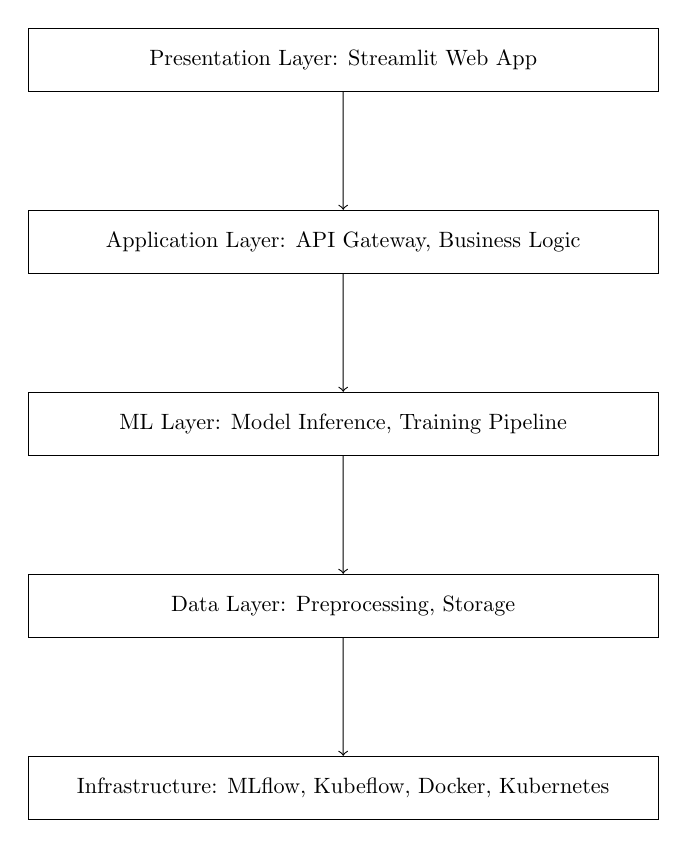
\begin{tikzpicture}[node distance=1.5cm, scale=0.8, every node/.style={scale=0.8}]
% Layers
\node[draw, rectangle, minimum width=10cm, minimum height=1cm] (presentation) {Presentation Layer: Streamlit Web App};
\node[draw, rectangle, minimum width=10cm, minimum height=1cm, below=of presentation] (application) {Application Layer: API Gateway, Business Logic};
\node[draw, rectangle, minimum width=10cm, minimum height=1cm, below=of application] (ml) {ML Layer: Model Inference, Training Pipeline};
\node[draw, rectangle, minimum width=10cm, minimum height=1cm, below=of ml] (data) {Data Layer: Preprocessing, Storage};
\node[draw, rectangle, minimum width=10cm, minimum height=1cm, below=of data] (infra) {Infrastructure: MLflow, Kubeflow, Docker, Kubernetes};

% Arrows
\draw[->] (presentation) -- (application);
\draw[->] (application) -- (ml);
\draw[->] (ml) -- (data);
\draw[->] (data) -- (infra);
\end{tikzpicture}
\caption{Layered Architecture Overview}
\label{fig:architecture}
\end{figure}

\subsection{Component Description}

\begin{enumerate}
    \item \textbf{End user Layer}:
    \begin{itemize}
        \item Streamlit web interface
        \item User input handling (image upload, face recognition)
        \item Results visualization
    \end{itemize}
    
    \item \textbf{ML Layer}:
    \begin{itemize}
        \item Model inference service (FaceNet, VGGFace, Custom CNN)
        \item Training pipeline orchestration
        \item Model versioning and registry
    \end{itemize}
    
    \item \textbf{Data Layer}:
    \begin{itemize}
        \item Face detection and preprocessing
        \item Data augmentation
        \item LFW dataset
    \end{itemize}
\end{enumerate}

\section{System Deployment \& Integration}

\subsection{Technology Stack}

\begin{table}[h]
\centering
\caption{Technology Stack}
\label{tab:tech_stack}
\begin{tabular}{|l|p{9cm}|}
\hline
\textbf{Layer} & \textbf{Technologies} \\
\hline
\textbf{Frontend} & Streamlit \\
\hline
\textbf{Backend} & Python \\
\hline
\textbf{ML Frameworks} & TensorFlow 2.x, PyTorch, Keras, scikit-learn \\
\hline
\textbf{Face Detection} & MTCNN, Dlib, OpenCV \\
\hline

\textbf{MLOps} & MLflow (tracking), Kubeflow (pipelines),  \\
\hline
\textbf{Deployment} & Hugging Face Spaces \\
\hline
\textbf{Version Control} & Git, GitHub \\
\hline
\end{tabular}
\end{table}
\newpage
\subsection{Deployment Diagram}

\begin{figure}[h]
\centering
\begin{tikzpicture}[node distance=2.5cm]
% Nodes (deployment components)
\node[deployment] (browser) {<<device>>\\User Browser};
\node[deployment, below=2cm of browser] (hf) {<<cloud>>\\Hugging Face\\Spaces};
\node[deployment, below=of hf] (streamlit) {<<container>>\\Streamlit App};
\node[deployment, below left=of streamlit] (model) {<<container>>\\Model Service};
\node[deployment, below right=of streamlit] (mlflow) {<<server>>\\MLflow Server};

% Connections
\draw[->] (browser) -- node[right] {HTTPS} (hf);
\draw[->] (hf) -- (streamlit);
\draw[<->] (streamlit) -- node[left] {Direct Call} (model);
\draw[<->] (streamlit) -- node[right] {Logging/Metrics} (mlflow);
\end{tikzpicture}
\caption{Deployment Diagram}
\label{fig:deployment}
\end{figure}

\newpage
\end{document}
